\subsection{Data}
The \verb+SUSY2+ derivation is used, where $\geq2$ light flavor leptons ($e$ or $\mu$) passing pre-selection are required. The selection details are:
\begin{itemize}
  \item $\mu$: $\pt>9$, $|\eta|<2.6$, \verb+DFCommonMuonsPreselection+
  \item $e$: $\pt>9$, $|\eta|<2.6$, \verb+Loose+ or \verb+DFCommonElectronsLHLoose+
\end{itemize}

\subsection{Signal Sample Grid}
\begin{figure}
  \centering
  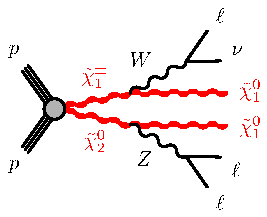
\includegraphics[width=0.35\textwidth]{C1N2-lllvN1N1-WZ}
  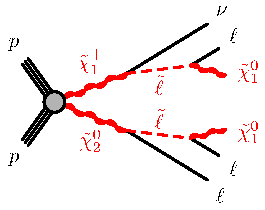
\includegraphics[width=0.35\textwidth]{C1N2-lllvN1N1-slsl}
  \caption{Deacy vis $\susy{l}$.}
  \label{fig_grid_sl}
\end{figure}
Grid infomation from $3l$ walkthrough note.
\begin{figure}
  \centering
  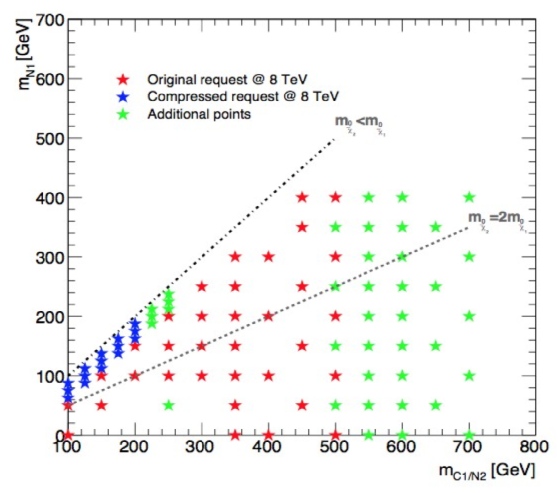
\includegraphics[width=0.49\textwidth]{C1N2_viaWZ3L_13TeC_newDesign}
  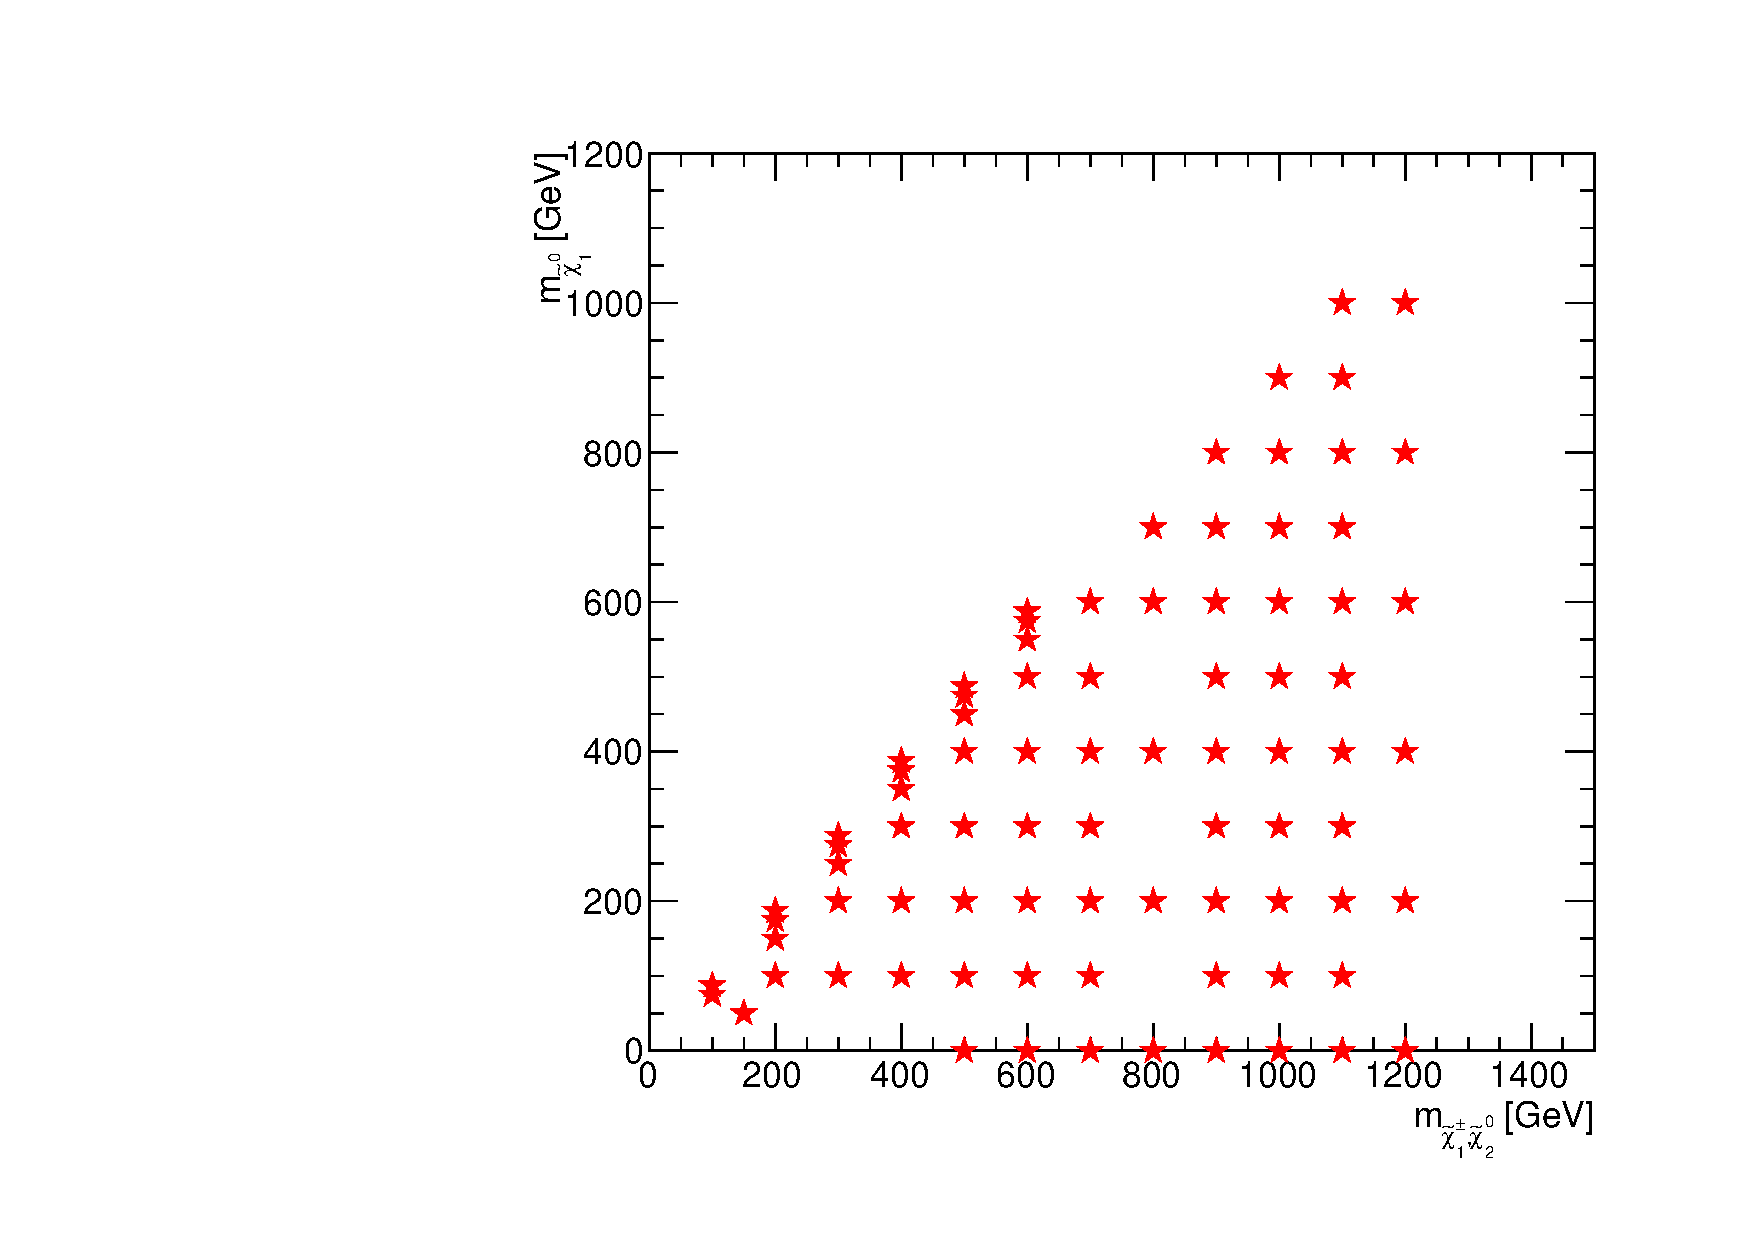
\includegraphics[width=0.49\textwidth]{C1N2_viaSL_13TeC_newDesign}
  \caption{Deacy vis $\susy{l}$.}
  \label{fig_grid_sl}
\end{figure}


The sample for $x=0.95$ mass splitting need to be requested.

\subsection{Background Simulation}
The description of the background MC.
